\chapter{Intermediate Algebra}

\section{Review and Expanding on Various Topics}

Phương trình một biến bậc nhất $ax+b=c$ có thể có: một nghiệm, vô nghiệm hoặc vô số nghiệm.

\vspace{.5cm}

\hl{Graphing Linear Inequalities}: Trong hình dưới, tất cả điểm được tô màu including the line đều thỏa mãn bất phương trình.

\begin{figure}[htb!]
  \centering
  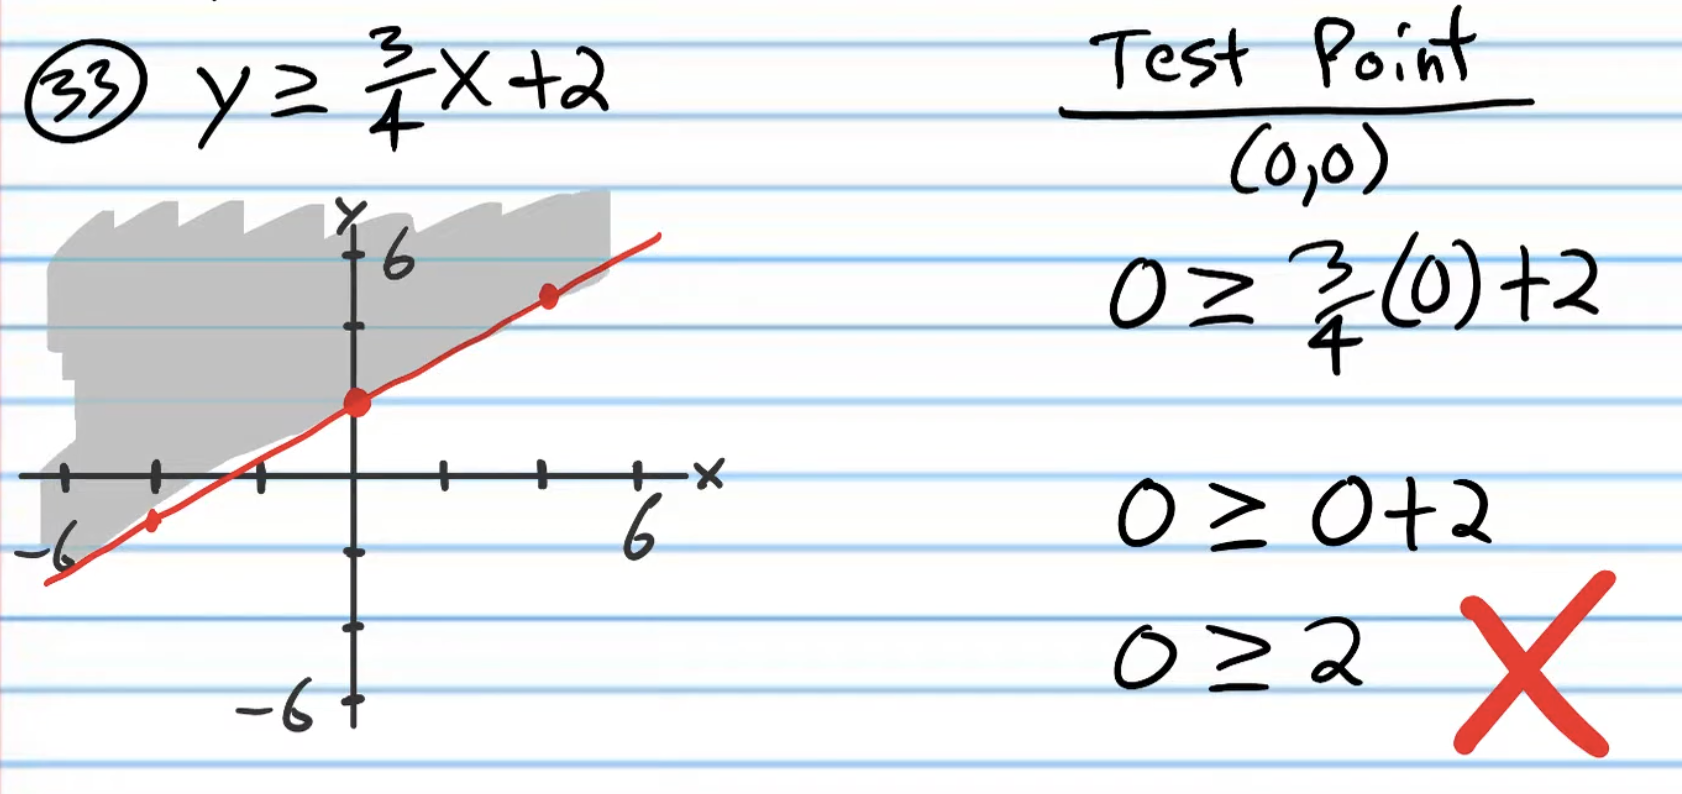
\includegraphics[width=.7\textwidth]{int0203.png}
  \caption{Graphing Inequalities}
\end{figure}

Draw the line giống như một linear equation, sau đó lấy tọa độ một điểm plug vào inequality để test coi phải tô màu phần nào. Thường chọn (0,0) cho dễ test. Nếu dựa vào greater thì tô màu phần trên, less than tô phần dưới là sai. Phải chọn test point.

\vspace{.5cm}

Draw (graph) \textbf{one variable inequality} like $2x-3>5$ thì sao? Linear Inequalities có x, y là 2D còn one variable x là 1D tức là một đường thẳng (the Number Line). Chấm một điểm rồi tô màu phần bên trái hay bên phải điểm đó thôi.

\vspace{0.6 cm}

\centerline{\textbf{\Large Graphing Systems of Linear Inequalities}}

\vspace{0.3 cm}

Two line intersect so four sections, only tô màu one section. Chọn test point phải chọn 3 điểm nằm trong 4 sections. Test point phải thỏa cả 2 bất phương trình.

Có equal thì sẽ full line, không thì vẽ dotted line.

\begin{figure}[htb!]
  \centering
  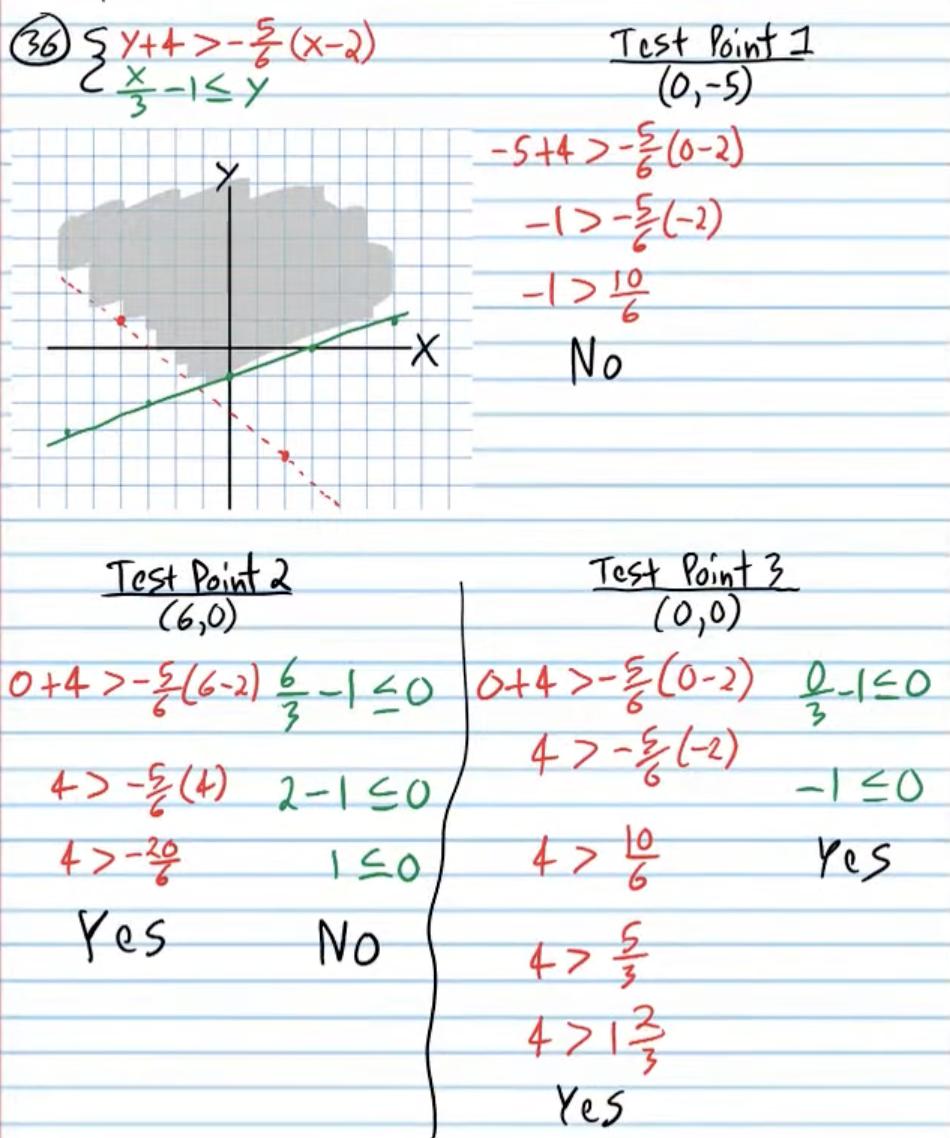
\includegraphics[width=.8\textwidth]{int0204.png}
  \caption{Graphing Systems of Linear Inequalities}
\end{figure}

\section{Solving Systems of Three Equations}

Hệ pt 3 biến cũng có tối đa một nghiệm (x, y, z), no solution, infinite solutions.

Tìm cách chuyển về hệ pt 2 biến x, y rồi giải.

Dùng substitution or elimination khử một ở 2 phương trình đầu biến nó thành hệ pt 2 biến x, y. Giải tìm x, y rồi sau đó tìm z.

\vspace{.4cm}

Bài ở dưới, khi lấy pt (a) cộng pt (c) ra $0=0$ là kết luận ngay \textbf{infinite solution}. Nhưng nếu tiếp tục làm ta sẽ phát hiện $x=1$ là constant và $y=z$ vô số nghiệm có dạng $(1, a, a)$.

\begin{figure}[htb!]
  \centering
  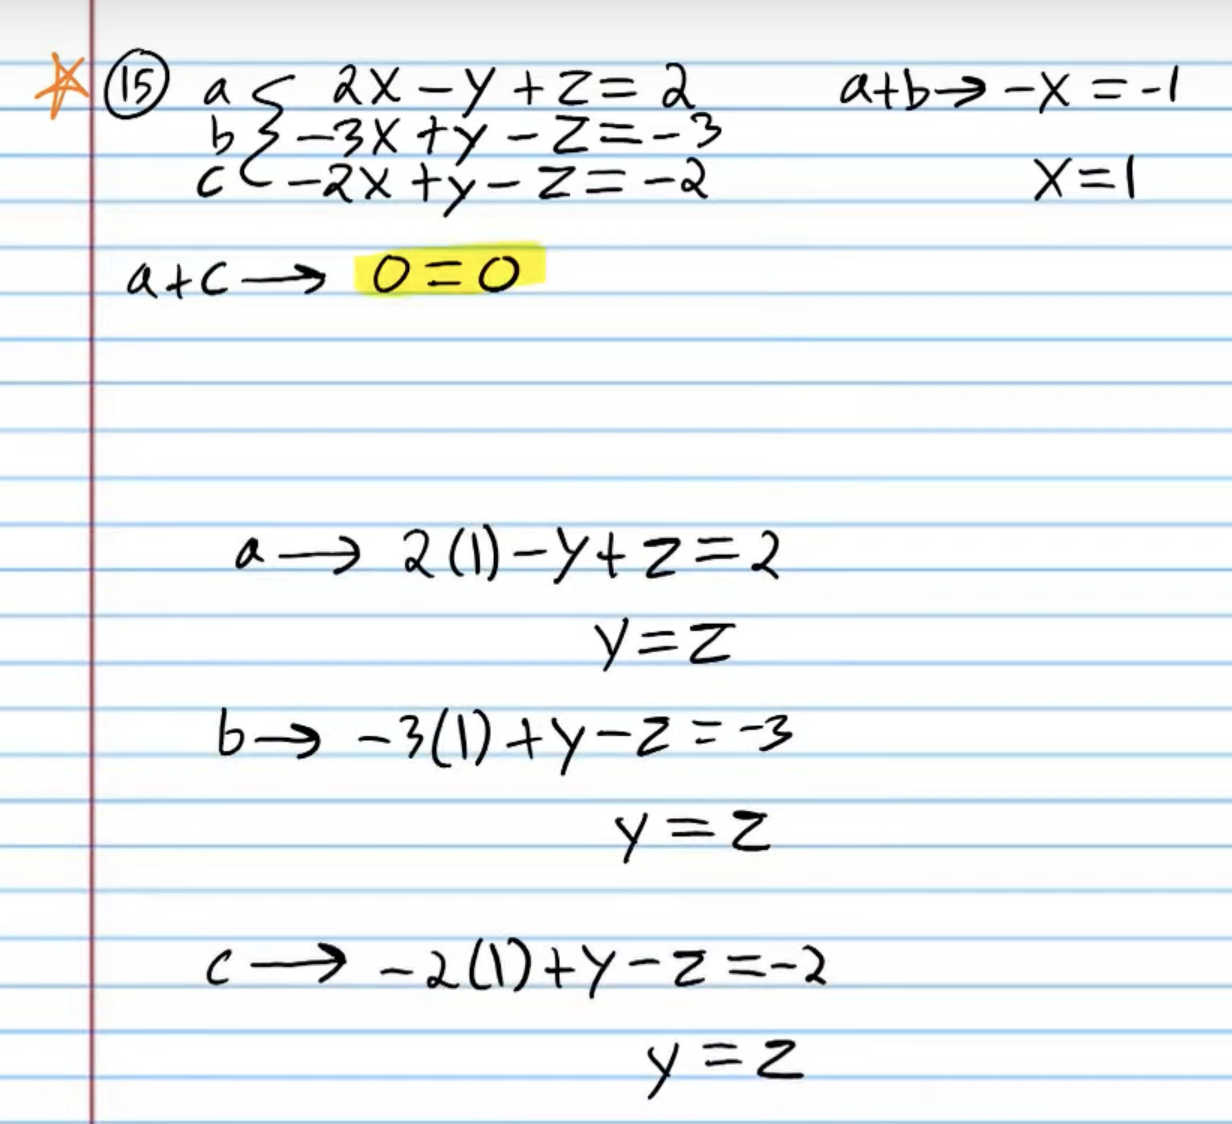
\includegraphics[width=.6\textwidth]{int0301.png}
  \caption{Bài tập}
\end{figure}

\section{Absolute Value Equations and Inequalities}
% 25 Aug 2025

\begin{multicols}{2}
[
%optional header
  \textbf{Exercise}: Solve these equations. \textit{Hint}: you always need to isolate the absolute values first.
]
\begin{equation*}
\begin{split}
  |x+2| &= 8 \\
  x+2=8 &\text{ or } x+2=-8\\
  x=6 &\text{ or } x=-10
\end{split}
\end{equation*}

\begin{center} \line(1,0){200} \end{center}

\begin{align*} 
|y|+2=-3\\
|y| = -5\\
  =>\text{ No Solution.}
\end{align*}

\begin{align*} 
  \frac{\left| \frac{b}{3}-4 \right|}{2} -5 &=-5\\
  \left| \frac{b}{3}-4 \right| &= 0 \\
  \frac{b}{3}-4 &=0 \text{ (không chia 2 trường hợp)}\\
  b&=12
\end{align*}

\end{multicols}

% https://tex.stackexchange.com/questions/19579/horizontal-line-spanning-the-entire-document-in-latex
% \noindent\rule{5cm}{0.4pt}
% \begin{center} \line(1,0){370} \end{center}
% \noindent\rule{\textwidth}{0.4pt}
% \hr

\vspace{0.6 cm}

\centerline{\underline{\textbf{\Large Absolute Value Inequalities}}}

\centerline{\textcolor{red}{(also called compound inequalities)}}

\vspace{0.3 cm}

You need to memorize these theorems below. Remember $|a| \text{ always } \geq 0$

\noindent\rule{\textwidth}{0.8pt}

\vspace{0.4 cm}

\centerline{\colorbox{orange}{\Large The Absolute Value Inequality Theorems}}

In the following inequalities, C is a nonnegative constant (including zero).

\begin{figure}[htb!]
  \centering
  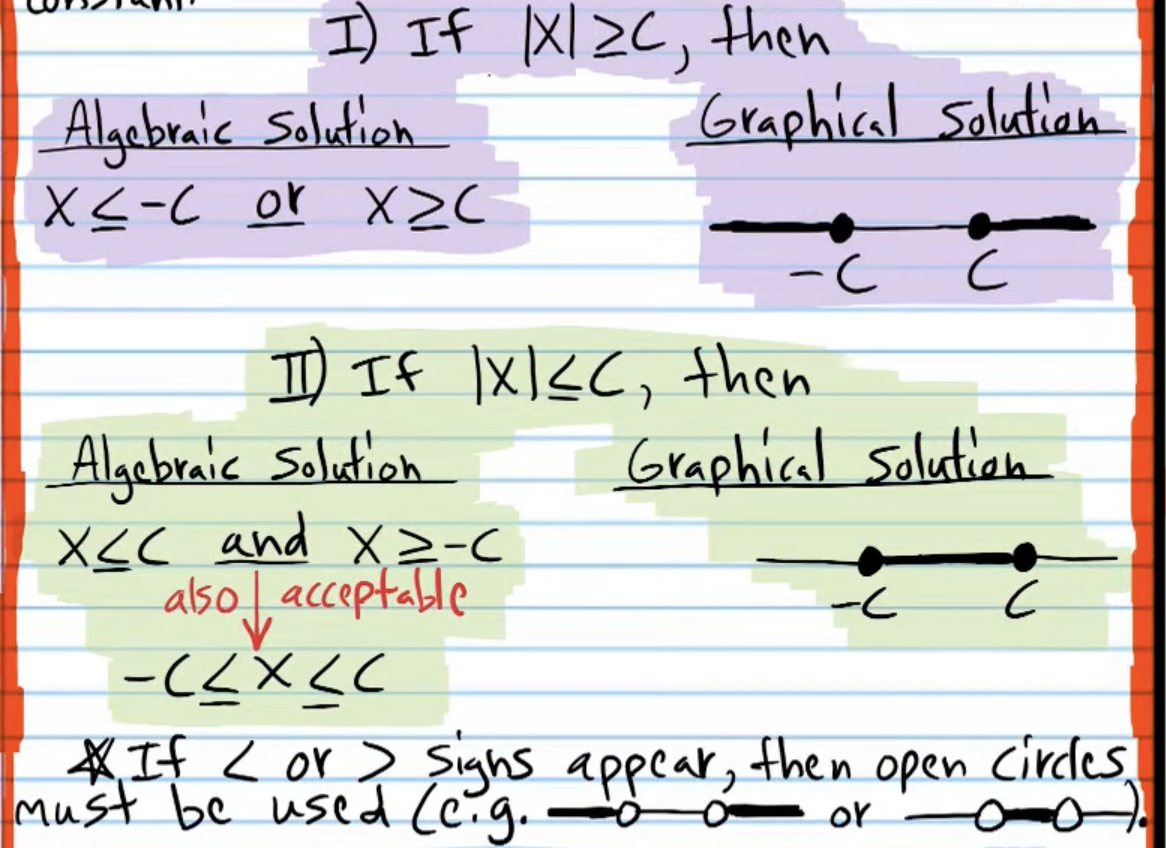
\includegraphics[width=.6\textwidth]{int0401.png}
  % \caption{Bài tập}
\end{figure}

\colorbox{SkyBlue}{III) If $|x|<-c$, then there are no solution.}

\colorbox{Thistle}{IV) If $|x| \leq 0$, then $x=0$ only.}

\colorbox{Aquamarine}{V) If $|x| \geq -c$, then x can be any real number.}

\colorbox{Lavender}{VI) If $|x| > 0$, then x can be any real number except zero.}

\noindent\rule{\textwidth}{0.8pt}

\begin{multicols}{2}
[
%optional header
  \textbf{Excercise}: Find the algebraic solutions \& the graphical solutions for the following inequalities.
]
\begin{align*}
  \circled{35}\ |x|&>2 \\
  x<-2 &\text{ or } x>2
\end{align*}

% \begin{center} \line(1,0){200} \end{center}

\begin{align*}
  \circled{47}\ 5&\geq \frac{|-2b-3|}{7}+2\\
  21&\geq |-2b-3| \\
  -21&\leq -2b-3 \leq 21\\
  9 &\geq b \geq -12
\end{align*}

\begin{align*}
  \circled{36}\ 7 &\geq |y|\\
  y \geq -7 &\text{ and } y \leq 7
\end{align*}

\begin{align*}
  \circled{48}\ 5|-2+6y|-8 &> 2\\
  |-2+6y|&>2\\
  -2+6y>2 \text{ or }& -2+6y<-2\\
  y>\frac{2}{3} \text{ or }& y<0
\end{align*}

\end{multicols}

\section{Roots - Part I}
% 27 Aug 2025

Roots are also called \textbf{Radicals}.

\textcolor{red}{{\LARGE $\star$} For all problems in this class, assume that all unknowns (variable x) are positive. Therefore, you do not have to use absolute value symbols when finding roots (e.g. $\sqrt{x^{2}}=|x|$).}

\begin{tcolorbox}[
  enhanced,attach boxed title to top center={yshift=-3mm,yshifttext=-1mm},
  colback=blue!5!white,colframe=blue!75!black,colbacktitle=red!80!black,
  title=Root Rules,fonttitle=\bfseries,
  boxed title style={size=small,colframe=red!50!black}
]
  \hspace{2cm}
  \colorbox{green}{$\sqrt{ab}=\sqrt{a}\sqrt{b}$}
  \hspace{7cm}
  \colorbox{green}{$\sqrt{\frac{a}{b}}=\frac{\sqrt{a}}{\sqrt{b}}$}
\end{tcolorbox}

\hl{Perfect Squares}: 1, 4, 9, 16, 25, 36, 49, 64, 81, 100

\vspace{.4cm}

\textbf{Excercise}: Factoring out a Perfect Square.

\begin{figure}[htb!]
  \centering
  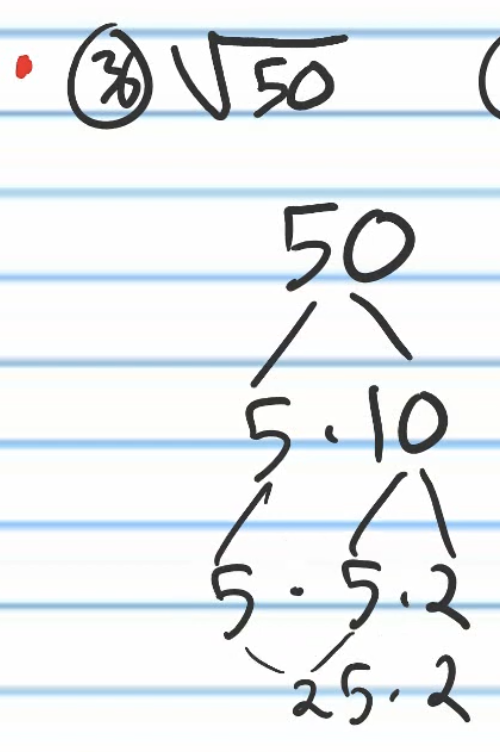
\includegraphics[width=.2\textwidth]{beg1401.png}
  % \caption{Bài tập}
\end{figure}

\[\circled{36}\ \sqrt{50}=\sqrt{25 \cdot 2}=5\sqrt{2}\]

Cách làm là construct a \textbf{Factor Tree} \& re-combine if you need to. This is not prime factorization but it's a similar idea.

\vspace{.4cm}

\begin{multicols}{2}
[
%optional header
  \textbf{Exercise}: Simplify these expressions.
]
\begin{align*}
  \circled{1}\ \sqrt{18x^{3}y^{2}}&= \sqrt{9 \cdot 2 \cdot x^{2} \cdot x \cdot y^{2}} \\
  &=3xy\sqrt{2x}
\end{align*}

% \begin{center} \line(1,0){200} \end{center}

\begin{align*}
  \circled{2}\ \sqrt{32x^{7}y^{3}}&=\sqrt{16\cdot 2 \cdot x^{6} \cdot x\cdot x^{2}\cdot y}\\
  &=4x^{3}y\sqrt{2xy}
\end{align*}

\begin{align*}
  \circled{4}\ \sqrt{16x^{10}y^{11}}=4x^{5}y^{5}\sqrt{y}
\end{align*}

\begin{align*}
  \circled{5}\ \sqrt{20x^{5}y}=2x^{2}\sqrt{5xy}
\end{align*}

\begin{align*}
  \circled{6}\ \sqrt{9x^{9}y^{6}}=3x^{4}y^{3}\sqrt{x}
\end{align*}

\begin{align*}
  \circled{7}\ \sqrt{12x^{2}y^{8}}&=2xy^{4}\sqrt{3}
\end{align*}

\begin{align*}
  \circled{8}\ \sqrt{25x^{6}y^{13}}&=\sqrt{25x^{6}y^{12}\cdot y}\\
  &=5x^{3}y^{6}\sqrt{y}
\end{align*}

\begin{align*}
  \circled{10}\ &-6\sqrt{4y^{4}}+10y^{2}-2\sqrt{81y^{2}}+17y\\
  &-12y^{2}+10y^{2}-18y+17y\\
  &-2y^{2}-y
\end{align*}

\begin{align*}
  \text{Example XII) }\ \frac{6}{\sqrt{50}}=\frac{6}{5\sqrt{2}}&=\frac{6\sqrt{2}}{10}\\
  &=\frac{3\sqrt{2}}{5}
\end{align*}

\begin{align*}
  \text{Example XXI) }\ \sqrt{\frac{5}{48}}=\frac{\sqrt{5}}{4\sqrt{3}}=\frac{\sqrt{15}}{12}
\end{align*}

\begin{align*}
  \text{Example XXV) }\ \frac{\sqrt{8}}{\sqrt{32}}=\sqrt{\frac{8}{32}}=\sqrt{\frac{1}{4}}=\frac{1}{2}
\end{align*}

\end{multicols}

Every even power (e.g. $x^{10}, $$x^{6}$, $x^{4}$, $x^{2}$) is a perfect square. You just divide the power by 2 when pulling it out of the square root ($\sqrt{x^{12}}=\sqrt{(x^{6})^{2}}=x^{12\div 2}=x^{6}$). Every odd power is NOT a perfect squarer.

\section{Roots - Part II}
% 30 Aug 2025 - lễ quốc khánh, trời mưa quá trời

\begin{multicols}{2}
[
%optional header
  \textbf{Exercise}: Rationalizing Two-Term Denominators
]

\begin{align*}
  \circled{1}\ \frac{3}{4+\sqrt{5}}&=\frac{3(4-\sqrt{5})}{(4+\sqrt{5})(4-\sqrt{5})}\\
  &=\frac{12-3\sqrt{5}}{11}
\end{align*}

\begin{align*}
  \circled{29}\ \frac{4}{\sqrt{x}-7}&=\frac{4(\sqrt{x}+7)}{(\sqrt{x}-7)(\sqrt{x}+7)}\\
  &=\frac{4\sqrt{x}-28}{x-49}
\end{align*}

\begin{align*}
  \circled{31}\ \frac{\sqrt{2}-3}{\sqrt{5x}+1}&=\frac{(\sqrt{2}-3)(\sqrt{5x}-1)}{(\sqrt{5x}+1)(\sqrt{5x}-1)}\\
  &=\frac{\sqrt{10x}-\sqrt{2}-3\sqrt{5x}+3}{5x-1}
\end{align*}

\begin{align*}
  \circled{3}\ \frac{2}{\sqrt{5}-6}&=\frac{2(\sqrt{5}+6)}{(\sqrt{5}-6)(\sqrt{5}+6)}\\
  &=\frac{2\sqrt{5}+12}{-31}
\end{align*}

\begin{align*}
  \circled{25}\ \frac{\sqrt{18x^{3}}}{\sqrt{32x^{9}}}&=\sqrt{\frac{9}{16x^{6}}}=\frac{3}{4x^{3}}
\end{align*}

\begin{align*}
  \circled{27}\ \frac{2}{\sqrt{x}+3}&=\frac{2(\sqrt{x}-3)}{(\sqrt{x}+3)(\sqrt{x}-3)}\\
  &=\frac{2\sqrt{x}-6}{x-9}
\end{align*}

\end{multicols}

We use the \hl{Fundamental Principle of Fractions} which states that multiplying or dividing both the numerator and the denominator by the same non-zero number creates an equivalent fraction, maintaining the original value.

\section{Roots - Part III: 3rd \& 4th roots}
%02 Sep 2025 nghĩ lễ quốc khánh 80 năm

\begin{tcolorbox}[
  enhanced,attach boxed title to top center={yshift=-3mm,yshifttext=-1mm},
  colback=blue!5!white,colframe=blue!75!black,colbacktitle=red!80!black,
  title=nth Root Rules,fonttitle=\bfseries,
  boxed title style={size=small,colframe=red!50!black}
]
  \hspace{2cm}
  \colorbox{green}{$\sqrt[n]{ab}=\sqrt[n]{a}\sqrt[n]{b}$}
  \hspace{6cm}
  \colorbox{green}{$\sqrt[n]{\frac{a}{b}}=\frac{\sqrt[n]{a}}{\sqrt[n]{b}}$}
\end{tcolorbox}

\hl{Perfect Cubes}: 1, 8, 27, 64, 125, 216, 343, 512, 729, 1000.

\vspace{.5cm}

\begin{multicols}{2}
[
%optional header
  \textbf{Exercise}: Simplify:
]

\begin{align*}
  \circled{4}\ \sqrt[3]{125}=5
\end{align*}

  \[\circled{5}\ \sqrt[3]{-216}=-6\]

  \[\circled{6}\ \sqrt[3]{-343}=-7\]

  \[\circled{7}\ \sqrt[3]{16}=\sqrt[3]{8\cdot 2}=2\sqrt[3]{2}\]

  \[\circled{9}\ \sqrt[3]{-80}=\sqrt[3]{-8\cdot 10}=-2\sqrt[3]{10}\]

  \[\circled{11}\ \sqrt[3]{-81}=\sqrt[3]{-27\cdot 3}=-3\sqrt[3]{3}\]

  \begin{align*}
    \circled{14}\ &\sqrt[3]{x^{9}}=x^{9\div 3}=x^{3}\\
    &\text{Because }x^{3}\cdot x^{3}\cdot x^{3}=x^{9}
  \end{align*}

  \[\circled{16}\ \sqrt[3]{x^{12}}=x^{12\div 3}=x^{4}\]

  \begin{align*}
    \circled{18}\ \sqrt[3]{x^{10}}&=\sqrt[3]{x^{9}\cdot x}=x^{3}\sqrt[3]{x}
  \end{align*}

  \begin{align*}
    \circled{21}\ \sqrt[3]{250x^{13}}&=\sqrt[3]{125\cdot 2\cdot x^{12}\cdot x}\\
    &=5x^{4}\sqrt[3]{2x}
  \end{align*}

  \begin{align*}
    \circled{22}\ \sqrt[3]{-40x^{6}}&=\sqrt[3]{-8\cdot 5 \cdot x^{6}}\\
    &=\sqrt[3]{-8}\cdot \sqrt[3]{5}\cdot \sqrt[3]{x^{6}}\\
    &=-2x^{2}\sqrt[3]{5}
  \end{align*}

  \begin{align*}
    \circled{29}\ &2\sqrt[3]{48x^{5}}-6x\sqrt[3]{-162x^{2}}\\
    &4x\sqrt[3]{6x^{2}}+18x\sqrt[3]{6x^{2}}\\
    &22x\sqrt[3]{6x^{2}}
  \end{align*}

  \begin{align*}
    \circled{31}\ \frac{-4}{\sqrt[3]{9}}=\frac{-4\cdot \sqrt[3]{3}}{\sqrt[3]{9}\cdot \sqrt[3]{3}}=\frac{-4\sqrt[3]{3}}{3}\\
  \end{align*}

  \begin{align*}
    \circled{32}\ \frac{8}{\sqrt[3]{5}}=\frac{8\cdot \sqrt[3]{25}}{\sqrt[3]{5}\cdot \sqrt[3]{25}}=\frac{8\sqrt[3]{25}}{5}
  \end{align*}

  \begin{align*}
    \circled{35}\ \frac{2}{\sqrt[3]{24}}&=\frac{2}{2\sqrt[3]{3}}=\frac{1}{\sqrt[3]{3}}=\frac{\sqrt[3]{9}}{3}
  \end{align*}

  \begin{align*}
    \circled{48}\ \sqrt[4]{x^{10}}=\sqrt[4]{x^{8}\cdot x^{2}}=x^{2}\sqrt[4]{x^{2}}
  \end{align*}

  \begin{align*}
    \circled{55}\ \sqrt[4]{\frac{2}{243x^{9}}}&=\frac{\sqrt[4]{2}}{\sqrt[4]{81\cdot 3 \cdot x^{8}\cdot x}}\\
    &=\frac{\sqrt[4]{2}}{3x^{2}\sqrt[4]{3x}}=\frac{\sqrt[4]{2}\cdot\sqrt[4]{27x^{3}}}{3x^{2}\sqrt[4]{3x}\cdot \sqrt[4]{27x^{3}}}\\
    &=\frac{\sqrt[4]{54x^{3}}}{9x^{3}}
  \end{align*}
\end{multicols}

Any power that is divisible by 3 is a perfect cube. You divide the power by the index 3 of the root when pulling it out of the cube root.

In \textbf{problem \#31}, we cannot multiply tử \& mẫu với $\sqrt[3]{9}$ được vì $\sqrt[3]{9\cdot 9}=\sqrt[3]{81}$ is not a perfect cube.

\section{Roots - Part IV: Negative Radicands, Imaginary Numbers, and Complex Numbers}
%4 Sep 2025

\begin{figure}[htb!]
  \centering
  
\includegraphics[width=.8\textwidth]{int0801.png}
  \caption{Roots Vocabulary}
\end{figure}

\vspace{0.5 cm}

\centerline{\underline{\textbf{\large Raising a Negative Number to an Even or Odd Power}}}

% \vspace{.5cm}

\begin{itemize}
  \item Even Powers Produce Positive Numbers: $(-2)^{2}=4$
  \item Odd Powers Produce Negative Numbers, Assuming that the Base is Negative: $(-2)^{3}=-8$
\end{itemize}

\vspace{0.3 cm}

\centerline{\underline{\textbf{\large \hl{Negative Variables under Radical Symbols}}}}

\begin{tcolorbox}[colback=red!5!white,colframe=red!75!black]
  If $x$ is NOT assumed to be positive, then \colorbox{green}{$\sqrt{x^{2}} \neq x$,but $\sqrt{x^{2}}=|x|$}, and if the index (n) of a root ($\sqrt[n]{x}$) is even, then there are other examples where absolute value symbols \textbf{must} be used.
\end{tcolorbox}

Lấy ví dụ $x=-5$, nếu viết $\sqrt{x^{2}}=x$ mà không có dấu absolute thì ta có $\sqrt{(-5)^{2}}=-5$ (wrong). The correct answer is $\sqrt{(-5)^{2}}=\sqrt{25}=5$. According to the order of operations (PEMDAS), you have to square inside part $(-5)^{2}=25$ first to get rid of the negative. Then you take the square root of positive 25. The absolute symbol makes sure that the answer is always a positive number even if the base of the radicand (x) is negative.

This rule is not related to the rule which states that \textbf{the even-index radical symbols can only produce a positive number} ($\sqrt{4}=2$ not -2 or $\sqrt[4]{81}=3$ not -3). While the \q{square root of 4} is 2 AND -2.

These two rules above, you must accept them. Don't ask question. The good news is this problem only occurs when you're dealing with even-index roots (2, 4, 6).

\vspace{.5cm}

\begin{multicols}{2}
[
%optional header
  \textbf{Exercise}: Simplify. \textcolor{red}{{\LARGE $\star$} Do NOT assume that the unknowns are positive.}
]

\begin{align*}
  \circled{1}\ \sqrt{x^{14}}=|x^{7}|
\end{align*}

  \[\circled{2}\ \sqrt[3]{x^{9}}=x^{3}\]

  \[\circled{3}\ \sqrt{x^{4}}=x^{2}\]

  \[\circled{4}\ \sqrt[5]{x^{5}}=x\]

  \[\circled{5}\ \sqrt[4]{x^{4}}=|x|\]

  \[\circled{6}\ \sqrt[4]{x^{16}}=x^{4}\]

  \[\circled{13}\ \sqrt{9x^{6}}=\sqrt{9}\cdot \sqrt{x^{6}}=3|x^{3}|\]
  
  \[\circled{15}\ \sqrt[4]{256x^{6}}=\sqrt[4]{256\cdot x^{4}\cdot x^{2}}=4|x|\sqrt[4]{x^{2}}\]

  \[\circled{17}\ \sqrt{49x^{10}}=7|x^{5}|\]

\end{multicols}

In problem \circled{3}, we don't need to put the absolute symbol because the answer $x^{2}$ is even-power so it is always positive. In problem \circled{1} however, we \textbf{must} use the absolute symbol because the answer $x^{7}$ is odd-power and CAN possibly be negative \textbf{IF} the base number $x$ is a negative number.

\vspace{0.5 cm}

\centerline{\underline{\textbf{\large \hl{Imaginary Numbers}}}}

% \vspace{.5cm}

\begin{align*}
  \iu&=\iu=\sqrt{-1}\ \text{ (Definition of i)}\\
  \iu^{2}&=(\sqrt{-1})^{2}=-1\\
  \iu^{3}&=i^{2}\cdot i=(-1)i=-\iu\\
  \iu^{4}&=i^{3}\cdot i=-i \cdot i=-i^{2}=-(-1)=1\\
  \iu^{5}&=i^{4}\cdot \iu=1\cdot i=i\ \text{ (\hyperref[fig:imaginary_pattern]{the pattern} repeat)}
\end{align*}

Example: $\iu,\ -5\iu,\ 7\iu,\ \iu\sqrt{3},\ \pi\iu,\ \frac{1}{2}\iu$. You can multiply $\iu$ by a number to get an imaginary number.

Cái này có luật chơi của riêng nó, không giống những rule mình học.

\vspace{0.5 cm}

\centerline{\underline{\textbf{\large \hl{Complex Numbers}}}}

\begin{figure}[htb!]
  \centering
  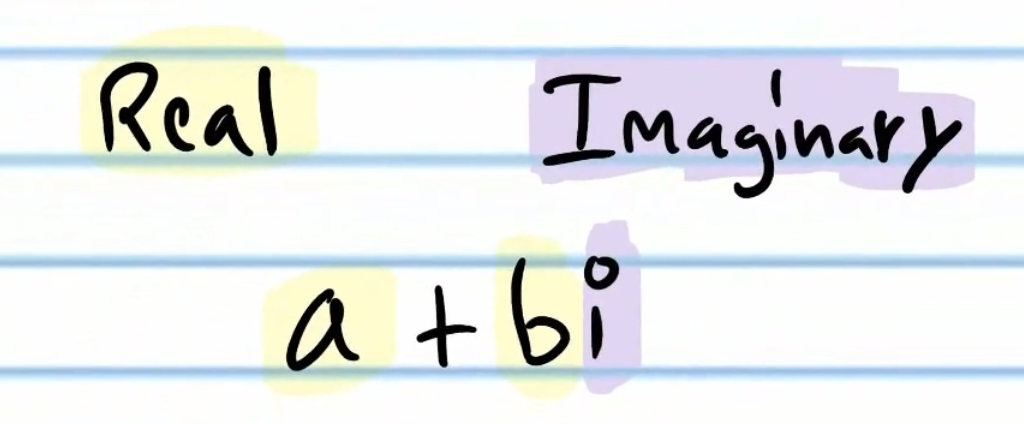
\includegraphics[width=.6\textwidth]{int0802.png}
  \caption{Complex Numbers}
\end{figure}

Example: $5+3\iu,\ -4+\iu,\ \sqrt{7}-2\iu,\ -9-\iu\sqrt{8},\ \frac{3}{4}+\frac{5}{7}\iu,\ \pi+2\iu,\ 10,\ 6\iu,\ \iu$.

The number 10 has no imaginary part. It is still considered a complex number.

\vspace{.5cm}

\begin{multicols}{2}
[
%optional header
  \textbf{Exercise}: Simplify.
]

\begin{align*}
  \circled{21}\ (5+2i)+(-1+3\iu)=4+5i
\end{align*}

  \begin{align*}
    \circled{25}\ &(-6+3i)-(4-9i)\\
    &-6+3i+(-4)+9i\\
    &-10 +12i
  \end{align*}

  \[\circled{29}\ 3i(4i)=12i^{2}=12(-1)=-12\]

  \[\circled{31}\ -7i(4i)=-28i^{2}=-28(-1)=28\]

  \begin{align*}
    \circled{32}\ 5i(3+8i)&=15i+40i^{2}\\
    &=15i+40(-1)\\
    &=-40+15i
  \end{align*}

  \[\circled{36}\ 3i(-2i)=-6i^{2}=-6(-1)=6\]

  \begin{align*}
    \circled{41}\ (4-2i)(5+3i)&=20+12i-10i-6i^{2}\\
    &=20+2i-6(-1)\\
    &=26+2i
  \end{align*}

  \begin{align*}
    \circled{47}\ (6+4i)^{2}&=36+48i+16i^{2}\\
    &=20+48i\\
  \end{align*}

  \begin{align*}
    \circled{48}\ (2-3i)^{2}&=4-12i+9i^{2}\\
    &=-5-12i\\
  \end{align*}

  \begin{align*}
    \circled{49}\ \frac{2}{3+i}&=\frac{2(3-i)}{(3+i)(3-i)}=\frac{6-2i}{9-i^{2}}\\
    &=\frac{6-2i}{9-(-1)}=\frac{6-2i}{10}\\
    &=\frac{6}{10}-\frac{2i}{10}=\frac{3}{5}-\frac{1}{5}i\ \text{ (**)}
  \end{align*}

  \begin{align*}
    \circled{50}\ \frac{-8}{2-5i}&=\frac{-8(2+5i)}{(2-5i)(2+5i)}=\frac{-16-40i}{4-25i^{2}}\\
    &=\frac{-16-40i}{29}=-\frac{16}{29}-\frac{40}{29}i\\
  \end{align*}

  \begin{align*}
    \circled{53}\ \frac{4+i}{-2+i}&=\frac{(4+i)(-2-i)}{(-2+i)(-2-i)}=\frac{-8-6i-i^{2}}{4-i^{2}}\\
    &=\frac{-8-6i-(-1)}{4-(-1)}=\frac{-7-6i}{5}\\
    &=-\frac{7}{5}-\frac{6}{5}i\\
  \end{align*}

  \begin{align*}
    \circled{57}\ \frac{2-8i}{3i}&=\frac{(2-8i)(i)}{3i\cdot i}=\frac{2i-8i^{2}}{3i^{2}}\\
    &=\frac{2i-8(-1)}{3(-1)}=\frac{2i+8}{-3}\\
    &=-\frac{8}{3}-\frac{2}{3}i
  \end{align*}
\end{multicols}

Problem \circled{41} is mutiplying two complex numbers. Cứ nhân phân phối (FOIL) bình thường như multiplying two binomials.

In Problem \circled{49}, we want complex numbers to be written in the \hl{$a+bi$} form. Đầu tiên ta nhân liên hợp (complex conjugate) để khử $i$ ở mẫu. Sau đó ở dòng (**), ta làm phép \textbf{fraction decomposition} to break the fraction into two parts.

% \vspace{.5cm}

% \threestars
\noindent\rule{\textwidth}{0.8pt}

For the problems below, use the pattern.

\begin{figure}[htb!]
  \centering
  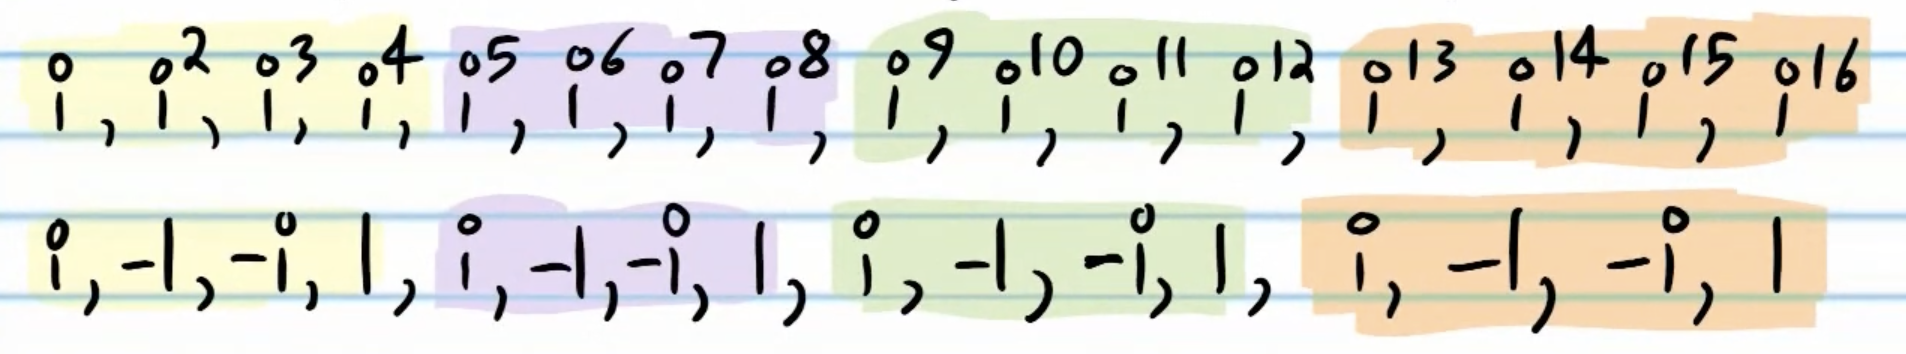
\includegraphics[width=.7\textwidth]{int0803.png}
  \caption{Imaginary patterns}
  \label{fig:imaginary_pattern}
\end{figure}

\textcolor{red}{{\LARGE $\star$} Hint}: Divide the power by four:

\begin{enumerate}
  \item \colorbox{cyan}{If the remainder\\ is zero, then the answer is 1.}
  \item \colorbox{green}{If the remainder is one, then the answer is $\iu$.}
  \item \colorbox{yellow}{If the remainder is two, then the answer is -1}
  \item \colorbox{magenta}{If the remainder is three, then the answer is $-\iu$.}
\end{enumerate}

\begin{multicols}{2}
[
%optional header
  \textbf{Exercise}: Simplify.
]

\begin{align*}
  \circled{21}\ (5+2i)+(-1+3\iu)=4+5i
\end{align*}
\end{multicols}
